L'analyse syntaxique permet de vérifier que la structure d'un programme est bien en accord avec les règles de grammaire du langage. Par exemple, la grammaire de notre langage comporte une règle qui indique que le jeton \verb|<FD>| doit être suivi d'un jeton \verb|<NUMBER,>|. Le but de notre analyse ici est double~: vérifier que le programme est bien un programme de notre langage valide, mais également généré un arbre abstrait qui pourra facilement être analysé par notre analyseur sémantique.

Nous avons fait le choix d'utiliser GNU Bison (cf.~\ref{bison}) dans notre projet.

\subsection{Arbre abstrait}
Un arbre abstrait est une structure d'arbre dont chaque noeud feuille représente les opérandes des opérations contenues sur les autres noeuds. Cet arbre peut être considéré comme une forme de code intermédiaire, et peut être interprété très facilement en interprétant pour chaque noeud, les sous-arbres et en appliquant l'opération du noeud courant.

\begin{figure}[h!]
\centering
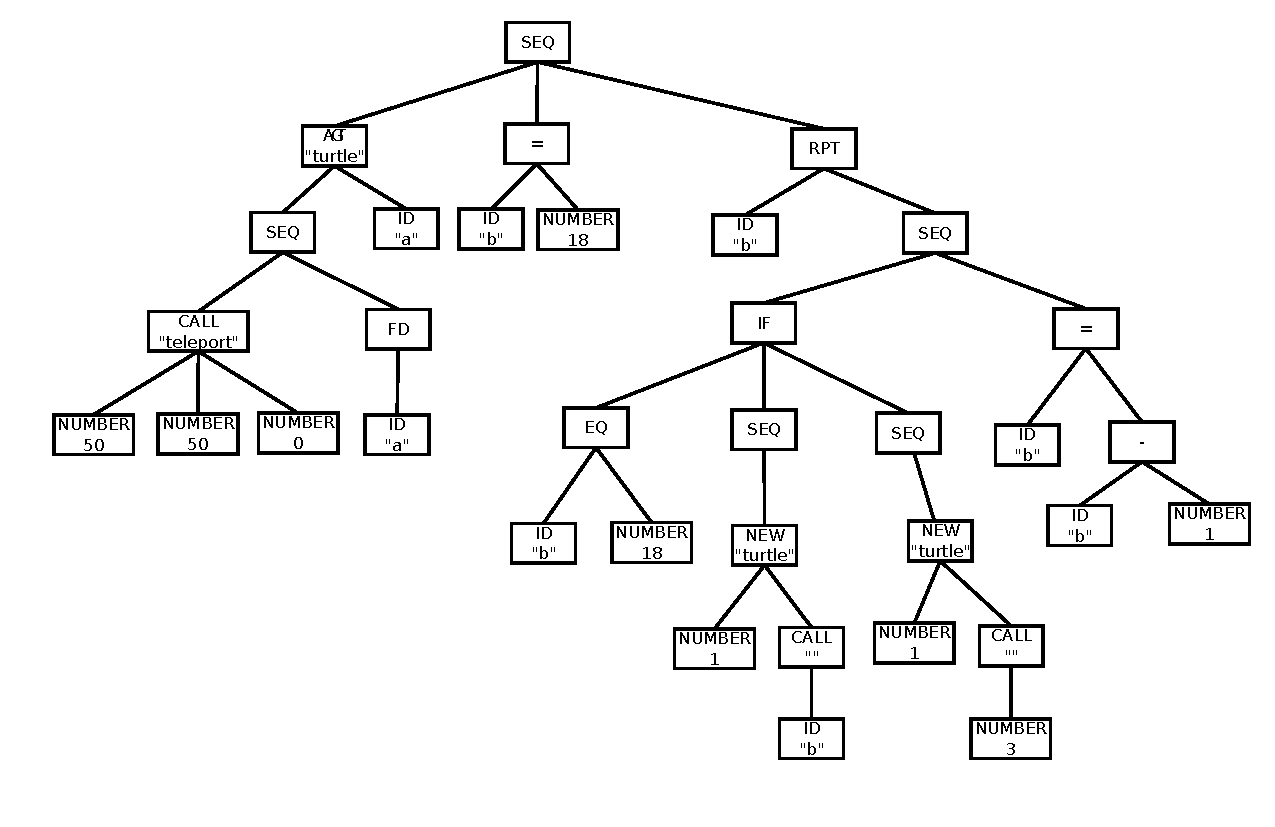
\includegraphics[scale=0.8]{doc/report/img/arbre-abstrait}
\caption{\label{arbre-abstrait} Arbre abstrait généré lors de l'analyse du code \ref{arbre-code}}
\end{figure}
\begin{lstlisting}[language=Stibbons,label=arbre-code,caption=Exemple de code Stibbons]
  agent turtle (a) {
    teleport(50,50,0)
    fd a
  }

  b = 18
  repeat b {
    if(b == 18) {
      new turtle(b)
    }
    else {
      new turtle(3)
    }
    b = b - 1
  }
\end{lstlisting}

L'avantage de générer un tel arbre est qu'il est bien plus rapide d'effectuer un parcours d'arbre à chaque interprétation plutôt que de refaire une analyse syntaxique à chaque fois.

\subsection{Fonctionnement}
L'écriture du fichier Bison est assez semblable au fichier Flex. En effet, on peut associer pour chaque règle une liste d'instructions qui vont être exécutées lors de la détection de la règle. Ces instructions peuvent en outre être des affectations de valeur sémantique à une expression. Ainsi, dans l'extrait de code \ref{bison-extrait}, la valeur sémantique d'une sélection est un arbre dont les enfants sont dans l'ordre~: l'expression de test, la séquence d'instructions à exécuter si la condition est vrai et, optionnellement, la séquence d'instructions à exécuter si la condition est fausse.

\begin{lstlisting}[label=bison-extrait,caption=Cas du IF en Bison]
selection : IF expr statement 
{
  stibbons::TreePtr t1 = make_shared<stibbons::Tree>(yy::parser::token::IF,nullptr);
  t1->addChild($2);
  t1->addChild($3);
  t1->setPosition({@1.begin.line,@1.begin.column});
  $$ = t1;
}
| IF expr statement ELSE statement
{
  stibbons::TreePtr t1 = make_shared<stibbons::Tree>(yy::parser::token::IF,nullptr);
  t1->addChild($2);
  t1->addChild($3);
  t1->addChild($5);
  t1->setPosition({@1.begin.line,@1.begin.column});
  $$ = t1;
};
\end{lstlisting}

Bison génère à partir de ces règles un analyseur syntaxique LALR (\emph{look-ahead left-to-right rightmost derivation}). L'analyse du code et la génération de l'arbre sont lancées par un appel à la méthode \verb|stibbons::Parser::parse()| qui va elle-même faire appel à la méthode \verb|yy::parser::parse()|. L'ensemble du code va être analysé, cette méthode se chargeant de faire appel à la méthode \verb|stibbons::FlexScanner::yylex()|, générant et analysant les jetons en une seule passe.
